\chapter{Grundlagen}

In diesem Kapitel werden die Grundlagen, welche für das weitere Verständnis der Arbeit und der
gesamten Anwendung notwendig sind, näher beschrieben. Zunächst werden die verschiedenen Technologien und Frameworks, sowohl des Frontends, als auch des Backends dargestellt. Anschließend werden einige gängige Angriffstypen im \ac{WWW} erläutert.

\section{Frontend Technologien und Frameworks}

Dieser Abschnitt behandelt alle notwendigen Technologien, die die grafische Darstellung von
Webinhalten und Interaktionen des Benutzers in seinem Browser ermöglichen. Da es sich bei \textit{webifier} um
eine Webanwendung handelt, sind dies ausschließlich Webtechnologien, welche von grafischen Browsern
unterstützt werden.

Die grundlegende Informationssprache des \ac{WWW} heißt \ac{HTML}. Sie wurde ursprünglich entwickelt
um wissenschaftliche Dokumente semantisch zu beschreiben (engl. 'to mark up'). Heute wird sie
jedoch in weitaus größerem Umfang genutzt.\footcite[Vgl.][]{html5Spec} \ac{HTML}-Dateien bestehen
aus zwei Arten von Informationen: Textdaten und Markupinformationen.
Erstere sind verantwortlich für den textuellen Inhalt der Webseite. Dazu zählen alle abgebildeten
Texte wie sie auch in Überschriften, Abschnitten, Menüs, usw. stehen. Sie sind die Informationen,
die Betrachter der Webseite direkt über das grafische Browserfenster lesen können.
Markupinformationen hingegen definieren den Aufbau und die Semantik der Inhalte. Diese sind für den
normalen Betrachter nicht unbedingt sichtbar. Hierbei handelt es sich um sogenannte Tags,
die im Quellcode in spitzen Klammern stehen und aus einer Menge von bestimmten Werten stammen. Tags
treten immer in Paaren auf, wobei der zweite Tag (Endtag) zusätzlich einen Backslash zwischen
aufgehender spitzer Klammer und Tagnamen hat (Listing \ref{lst:Beispiel.html} Zeile 5).
Innerhalb dieser beiden Tags können wiederum neue Tags, aber auch einfache Textdaten stehen (siehe
Zeile 4).
Diese Verschachtelung führt dazu, dass meist ein komplexer Baum von Tagelementen entsteht. Zu den
wichtigsten Tags zählt der \lstinline[style=eclipse]{<html>}-Tag. Er ist der äußerste Wurzeltag,
der alle anderen Tags umschließt. \lstinline[style=eclipse]{<head>}- und
\lstinline[style=eclipse]{<body>}-Tag stehen beide eine Ebene tiefer und beinhalten Metadaten für
das gesamte Dokument bzw. den Seiteninhalt.\footcite[Vgl.][57]{webTechnologies}

\begin{scriptsize}
\lstset{
    style=eclipsehtml,
    caption={Beispiel.html},
    label={lst:Beispiel.html}
}
\begin{lstlisting}
<!DOCTYPE html>
<html>
<head>
	<title>Testseite</title>
</head>
<body>
	<h1>Überschrift</h1>
	<p>Abschnitt 1</p>
	<p>Abschnitt 2</p>
</body>
</html>
\end{lstlisting}
\end{scriptsize}

Um den in \ac{HTML} definierten Inhalt optisch ansprechend zu gestalten verwenden Webseiten \ac{CSS}.
\ac{CSS} ist eine deklarative Sprache, mit der sich alle Optik-relevanten Eigenschaften von \ac{HTML}-Elementen definieren lassen, die dann vom Browser entsprechend angezeigt werden.
Die einfachste Möglichkeit ist es, die gewünschten Änderungen direkt über das \lstinline[style=eclipse]{style}-Attribut des jeweiligen Elements anzugeben.
Dazu wird die zu ändernde Eigenschaft angegeben, gefolgt von einem Doppelpunkt und dem neuen
Eigenschaftswert.
Alle Anweisungen sind durch ein Semikolon zu trennen.
Um die gleichen Änderungen auf mehrere Elemente anzuwenden, sollten diese Anweisungen in einem globalen Stylesheet zu einem Regelset gebündelt werden.
Stylesheets können direkt im \ac{HTML} in ein Style-Element als Textwert angegeben
(Listing \ref{lst:Beispiel.css} Zeilen 5 - 9), oder über ein Link-Element zu einer
\ac{CSS}-Datei nachgeladen werden.
In beiden Fällen ist es notwendig anzugeben, auf welche Elemente diese Regeln angewandt werden sollen.
Dies geschieht über den \ac{CSS}-Selektor.
Er wird vom Browser interpretiert und kann verschiedene Einschränkungen auf die Menge der betroffenen Elemente machen.
Häufige Kriterien der Selektoren sind Elementnamen, IDs und Klassennamen.
Elementnamen werden unformatiert angegeben. IDs werden durch eine vorangestellte Raute und
Klassennamen durch einen vorangestellten Punkt markiert (Listing \ref{lst:Beispiel.css} Zeile
7ff).
Mehrere Selektoren werden durch Kommas getrennt.
Weiterhin können Kindschaftsverhältnisse, Pseudoklassen und Nachbarschaften in Selektoren verwendet werden um komplexere Regelwerke zu definieren.
\footcite[Vgl.][125\psq]{webTechnologies}

\begin{scriptsize}
\lstset{
	style=eclipsehtml,
	caption={Beispiel.css},
	label={lst:Beispiel.css}
}
\begin{lstlisting}
<!DOCTYPE html>
<html>
<head>
	<title>Testseite</title>
	<style>
	body { background-color: grey }
	#datum { text-decoration: underline }
	.abschnitt { font-size: 20px }
	</style>
</head>
<body>
	<h1 style="color: red">Überschrift</h1>
	<span id="datum">08.07.2017</span>
	<p class="abschnitt">Abschnitt 1</p>
	<p class="abschnitt">Abschnitt 2</p>
</body>
</html>
\end{lstlisting}
\end{scriptsize}

\label{par:javascript}
JavaScript ist die Sprache, die den Inhalt von Webseiten lokal interaktiv macht.
Sie ist eine leichtgewichtige, objektorientierte und dynamisch schwach typisierte Skriptsprache, die von Browsern interpretiert wird.
Ihre Syntax erinnert stark an C und C++.
Ähnlich wie bei \ac{CSS} gibt es die Möglichkeit JavaScript direkt im \ac{HTML}-Dokument zu schreiben.
Dies geschieht über das \lstinline[style=eclipse]{<script>}-Element.
Der auszuführende Code wird direkt als Textwert angegeben.
Soll hingegen eine externe JavaScript-Datei eingebunden werden, so wird sie über das \lstinline[style=eclipse]{src}-Attribut referenziert.
\footcite[Vgl.][198]{webTechnologies}
Die Hauptaufgaben, die in JavaScript erledigt werden sind die Reaktion auf Nutzereingaben durch
Events, Modifikation des Webseiteninhalts und die asynchrone Kommunikation mit Webservern.

\label{par:jquery}
Um diese Aufgaben für mehrere Browser einheitlich und pragmatisch zu lösen, wurde die  Bibliothek \textit{jQuery} entwickelt.
\footcite[Vgl.][]{jqueryHomepage}
Der Einstiegspunkt von \textit{jQuery} ist die \lstinline[style=eclipse]{$}-Funktion.
Wird sie mit einem \ac{CSS}-Selektorstring als Parameter aufgerufen, so interpretiert sie ihn und liefert alle passenden \ac{HTML}-Elemente als Menge von \textit{jQuery}-Objekten zurück.
Durch die Struktur des \textit{jQuery}-\ac{API} können auf dieser Ergebnismenge direkt neue
Funktionen aufgerufen werden, die intern auf jedes Objekt einzeln angewandt werden.
Dieses Verhalten findet sich in vielen weiteren Funktionen von \textit{jQuery} wieder und erlaubt viele verkettete Funktionsaufrufe in einer einzigen Anweisung.
Weiterhin vereinfacht \textit{jQuery} die Erstellung von Elementen.
Wird die \lstinline[style=eclipse]{$}-Funktion mit einem \ac{HTML}-Tagstring (z.B.
\lstinline[style=eclipse]{$("<div>")}) aufgerufen, so wird dadurch ein \textit{jQuery}-Objekt
erstellt, dass das entsprechende Element repräsentiert.
Dieses Objekt kann nun weiter durch Funktionen modifiziert werden, indem Attributwerte gesetzt
und Routinen für Interaktionsereignisse definiert werden.
Beim Einfügen des Elements in das Dokument, kann wieder die \lstinline[style=eclipse]{$}-Funktion verwendet werden um den Vaterknoten zu bestimmen und ihm das generierte Element anzuhängen.
Die Schlichtheit, die Verkettungsmöglichkeit und das Prinzip der Mengenoperationen von \textit{jQuery} spart Entwicklern Platz und macht zusammengehörige Anweisungen besser lesbar.
\footcite[Vgl.][3\psqq]{jqueryReference}
Aus diesen Gründen setzen viele Webentwickler auf diese Bibliothek.
In den neuen Versionen von JavaScript werden diese Features allerdings auch teilweise
implementiert, sodass sich der Mehrwert etwas verringert und kritischer überlegt werden sollte, ob
die Nachteile der Abhängigkeit gegenüber dem Mehrwert gering genug sind.

Da sich \textit{webifier} an unerfahrene Internetnutzer wendet liegt ein Schwerpunkt auf
einem professionellen \ac{UI}, einer optimalen Usability und auf einer User Experience, die dem
Nutzer ein Gefühl von Sicherheit gibt.
Um diese nichtfunktionalen Anforderungen an die Oberfläche einheitlich und korrekt umzusetzen verwendet die Webanwendung das \ac{UI}-Framework \textit{Bootstrap}.
Das Framework wurde 2010 von einem Designer und einem Entwickler der Social Media Plattform Twitter erschaffen.
\footcite[Vgl.][1]{bootstrap}
Damals wurde es als ein interner Styleguide zur Standardisierung von Oberflächen verwendet.
Heute ist es ein sehr bekanntes Open Source Projekt und eines der führenden Webframeworks in ebendiesem Bereich.
\textit{Bootstrap} liefert neben den grundlegenden \ac{CSS}-Regeln für Standardelemente auch ein Strukturierungssystem mit, das es Entwicklern ermöglicht ihre Webseiten für alle möglichen Endgeräte mit verschiedenen Auflösungen zu optimieren.
Dieses Prinzip nennt sich \textit{Responsive Design} und lässt sich in \textit{Bootstrap} durch
\ac{CSS}-Regeln an die eigenen Anforderungen anpassen.
\footcite[Vgl.][7\psq]{bootstrap}
Im Kern wird \textit{Bootstrap} so verwendet, dass die zu vereinheitlichenden Elemente mit Framework-spezifischen Klassennamen versehen werden.
\footcite[Vgl.][4]{bootstrap}
Zusätzlich zu der einheitlichen \ac{UI} und dem Repsonsive Design können mit dem Framework auch
häufig gebrauchte Interaktionsmuster durch \ac{HTML}-Code angegeben werden.
Dazu muss das JavaScript-Paket als Ressource angegeben werden, wobei diese wiederum eine kompatible
Version von \hyperref[par:jquery]{jQuery} voraussetzt.

\section{Backend Technologien und Frameworks}

In diesem Abschnitt werden alle Technologien und Frameworks vorgestellt welche in den Backends der einzelnen Teilanwendungen zum Einsatz kamen.

\label{par:java}
Wohl am häufigsten kam die Programmiersprache Java zum Einsatz. Java ist eine universal einsetzbare,
nebenläufige, klassenbarierte und objektorientierte Programmiersprache. Sie wurde möglichst einfach
gestaltet um von vielen Entwicklern genutzt zu werden. In ihrer Syntax ähnelt sie den
Programmiersprachen C und C++. Außerdem ist sie stark und statisch typisiert. Vorallem aber
zeichnet sich Java durch seine Plattformunabhängigkeit aus. Diese wird dadurch umgesetzt, dass
Java-Quellcode in plattformunabhängigen Byte-Code kompiliert wird, welcher von einer \ac{JVM} ausgeführt wird. Java ist eine Hochsprache, die mit Hilfe des so genannten \enquote{Garbage Collectors} eine automatische Speicherverwaltung bereitstellt. \footcite[Vgl.][1]{javaspecification}

In einigen Teilprojekten wurde das auf Java basierende \textit{Spring}-Framework verwendet.
\textit{Spring} stellt eine vereinfachte Möglichkeit zum Zugriff auf viele \ac{API} der
Standard-Version zur Verfügung. Ein weiterer wesentlicher Bestandteil des
\textit{Spring}-Frameworks ist die \textit{Dependency Injection}. Hierbei suchen sich Objekte ihre
Referenzen nicht selbst, sondern bekommen diese anhand einer Konfiguration injiziert. Dadurch sind
sie eigenständig und können in verschiedenen Umgebungen eingesetzt werden. Des weiteren bringt
\textit{Spring} eine Unterstützung für aspektorientierte Programmierung mit, wodurch mit
verschiedenen Abstraktionsschichten einzelne Module abgekapselt werden können. \footcite[Vgl.][2]{spring3}

Aufbauend auf dem \textit{Spring} Basis-Modul werden noch weitere Module, wie beispielsweise Spring
Security, Sprint Boot, Spring Integration, Spring Data, Spring Session oder Spring MVC
bereitgestellt.
\footcite[Vgl.][2]{springPivotal} Im folgenden werden die \textit{Spring}-Mudule näher erläutert,
die für das weitere Verständnis der Arbeit notwendig sind.

\begin{description}
  \item[Spring Boot] \hfill \\
    Mit Spring Boot können Anwendungen, welche das \textit{Spring}-Framework nutzen, einfacher
    eintwickelt und ausgeführt werden, da dadurch eigenständig lauffähige Programme erzeugt werden können, welche nicht von externen Services abhängig sind. Hierfür bringt Spring Boot einen integrierten Server mit, auf welchem die Anwendung bereitgestellt wird.\footcite[Vgl.][1]{springBoot}
  \item[Spring MVC] \hfill \\
    Spring MVC ist sehr gut geeignet um Webanwendungen zu implementieren.\footcite[Vgl.][3]{spring3}
    Hierfür können diese in mehrere Abstraktionsschichten gegliedert werden, beispielsweise in
    \ac{UI}, Geschäftslogik und Persistenzschicht.\footcite[Vgl.][21]{springMvc}
  \item[Spring Data] \hfill \\
    Spring Data vereinfacht Datenbankzugriffe ungemein. Das Modul stellt \acp{API} für fast alle
    gängigen Datenbankzugriffsschichten, wie JDBC (Java Database Connectivity), Hibernate, JDO
    (Java Data Objects) zur Verfügung. Aber nicht nur relationale Datenbanken werden unterstützt,
    sondern beispielsweise auch NoSQL-Datenbanken und Key/Value-Stores können problemlos eingesetzt
    werden.\footcite[Vgl.][3f]{springData}
\end{description}

In Verbindung mit Spring Data wurde eine \textit{MongoDB} zur Speicherung der Ergebnisse
eingesetzt. \textit{MongoDB} ist eine dokumentorientierte, anpassungsfähige und skalierbare
Datenbank. Sie vereint viele nützliche Eigenschaften von relationalen Datenbanken, wie
Sekundärindizes, Auswahlabfragen und Sortierung mit Skalierbarkeit, MapReduce-Aggregationen und
raumbezogenen Indizes. Außerdem gibt es bei \textit{MongoDB} keine festen Schemata, weshalb großen
Datenmigrationen normal nicht notwendig sind.\footcite[Vgl.][1f]{mongodb}

Gewonnene und gespeicherte Daten müssen danach noch aufbereitet und visualisiert werden.
\textit{webifier} setzt dafür auf die Programmiersprache R. R ist eine freie Programmiersprache,
entwickelt für statistische Auswertungen und Visualisierungen. Sie zählt zu den prozeduralen
Programmiersprachen. Die quelltextoffene Sprache wird ständig weiterentwickelt.
Zusätzlich gibt es eine Vielzahl an Packages, welche weitere Funktionalität bereitstellen. Diese
sind über ein zentrales Repository abrufbar und so leicht in den Quelltext einzubinden.
\footcite[Vgl.][1ff]{R}

Ein wichtiger Bestandteil jedes großen Software-Projektes ist ein gutes Build-Management-Tool. Für
\textit{webifier} wurde \textit{Gradle} als solches gewählt. Ein Build-Prozess besteht grundsätzlich
aus zwei Teilschritten. Zum Einen aus dem Kompilieren des Codes und zum Anderen aus dem Verlinken
der benutzen Bibliotheken. \footcite[Vgl.][]{buildprozess} Da das manuelle Einbinden von
Bibliotheken und Kompilieren des Codes bei großen Projekten sehr aufwändig und mühsam sein kann
wird hier auf Build-Management-Tools wie \textit{Gradle} zurückgegriffen. Um den Build für den
Nutzer möglichst einfach zu gestalten verfolgt Gradle zwei Prinzipien. Das erste Prinzip ist
\textit{Convention over Configuration}, was bedeutet, dass soweit es geht ein Standardbuildprozess
definiert ist und der Anwender nur die Parameter ändern muss, die projektspezifisch abweichen. Das
zweite Prinzip nennt sich \textit{Don't Repeat Yourself}. Hierbei geht es darum Redundanzen in der
Konfiguration des Buildes zu vermeiden. Diese beiden Prinzipien helfen Gradle, dass meist kurze Build-Skripte ausreichen um komplexe Prozesse abzubilden. \footcite[Vgl.][6f]{gradle}

Die Kommunikation zwischen Server und Client erfolgt über \ac{REST}. Hierbei wird jedes Objekt als
Ressource definiert, welches über einen eindeutigen \ac{URI} adressiert werden kann. Über die
HTTP-Methoden GET, PUT, POST und DELETE können diese Ressourcen geladen, erstellt, geändert
oder auch gelöscht werden. \footcite[Vgl.][]{rest}

Das Testen von potenziell gefährlichen Webseiten soll natürlich nicht direkt auf dem Server
geschehen, da es diesen sonst potenziell gefährden könnte. Deshalb wird hierfür eine
Virtualisierung benötigt um die Tests abgekapselt vom Gesamtsystem auszuführen. Dafür wird Docker
als Tool eingesetzt. Docker ist eine Open-Source-Software zur Virtualisierung von Anwendungen.
Hierbei wird auf die Container-Technologie gesetzt. Container sind vom Betriebssystem
bereitgestellte isolierte Umgebungen zur Ausführung von Prozessen. Ein Vorteil der Container
gegenüber der herkömmlicher virtuelle Maschinen ist der vielfach geringere Ressourcenbedarf.\footcite[Vgl.][]{docker}

\section{Technologien und Frameworks der Tests}

In diesem Kapitel werden die notwendigen Technologien und Frameworks erläutert, die zur Umsetzung
der Sicherheitstests verwendet werden.

\textit{Python} ist eine skriptbasierte Interpretersprache und auf Integration von
verschiedenen Systemen spezialisiert.
Die Sprache wird von der Python Software Foundation nach Open Source Standards entwickelt.
Python zählt zu den dynamisch typisierten Programmiersprachen, was bedeutet, dass es wie bei \hyperref[par:javascript]{JavaScript} erst zur Laufzeit zu einer Typenprüfung kommt.
Weiterhin werden Codeblöcke nicht durch Sonderzeichen (wie z.B. geschweifte Klammern in Java)
gekennzeichnet, sondern definieren sich anhand der Einrückungstiefe.
\footcite[Vgl.][]{pythonHomepage}
Da Python ein bekanntes Open Soure Projekt ist, beteiligen sich viele Programmierer an der Entwicklung von Zusatzprogrammen, sogenannten \textit{Packages}.
Es gibt mittlerweile bereits über 100.000 Pakete\footcite[Vgl.][]{pypi}, die alle frei verfügbar sind und über einen einheitlichen Prozess in Projekte eingebunden werden können.
Aus diesen Flexibilitätsgründen und wird für die Testlogik in \textit{webifier} überwiegend Python verwendet.

\label{par:phantomjs}
Für eine automatisierte Webseitenanalyse wird der Browser \textit{PhantomJS} verwendet.
Dieser basiert auf der Browser Engine \textit{WebKit} der Firma Apple.
Da \textit{PhantomJS} ein headless Browser ist besitzt er keine grafische Benutzeroberfläche.
Er wird über JavaScript gesteuert und über eine ausführbare Datei aufgerufen.
Weitere Hauptfeatures sind: Bildschirmaufnahmen, Nutzersimulation und Netzwerküberwachung.
\footcite[Vgl.][]{phantomjs}
In \textit{PhantonJS} gilt es zwischen dem Steuerungsskript und dem Code der Webseite
zu unterscheiden.
Ersteres konfiguriert die Webseite und führt die Testlogik aus.
In der Testlogik können wiederum Anweisungen an die Webseite geschickt werden, die mit dem Rest des
Steuerungsskripts nichts zu tun haben. Sie haben einen eigenen Geltungsbereich, nämlich den in der
Browser Engine.

Um Webseiten mit all ihren Ressourcen herunterzuladen wurde die freie Software \textit{HTTrack}
verwendet. Mit \textit{HTTrack} können Webseiten in einem lokalen Verzeichnis gespeichert werden.
Hierfür erzeugt das Programm rekursiv alle notwendigen Verzeichnisse und lädt anschließend alle
Ressourcen, wie \ac{HTML}-, \ac{CSS}- und JavaScript-Dateien, sowie Bilder und andere Dateien
herunter. Außerdem ist es möglich automatisiert alle \ac{HTML}-Links entsprechend zu modifizieren.
Abschließend bietet \textit{HTTrack} umfassende Konfigurationsoptionen um es für den optimalen
Gebrauch anpassen zu können.\footcite[Vgl.][]{httrack}

Für die Analyse und den Vergleich von Bildern wurde auf die freie JavaScript-Bibliothek Resemble.js
zurückgegriffen. Mit Resemble können jegliche Arten von Bildanalyse und Bildvergleich genutzt
werden. Urspünglich wurde es für eine Bibliothek von \textit{Phantom JS} entwickelt, kann aber
inzwischen vielseitig eingesetzt werden. Resemble bietet einige Einstellungsmöglichkeiten um Bilder
analysieren und miteinander vergleichen zu können. Als Resultat liefert es bei der Bildanalyse
Helligkeits- und Farbwerte des Bildes. Beim Bildvergleich bekommt man den prozentualen Unterschied
der beiden Bilder, sowie einige Zusatzinformationen. Außerdem ist es möglich mit Resemble.js ein
Differenzbild mit der Hervorhebung der Unterschiede zweier Bilder zu erzeugen.\footcite[Vgl.][]{resemblejs}

Zu einer umfassenden Analyse gehört auch die Analyse des Netzwerktraffics. Dazu
wird ein entsprechendes Tool genutzt. \textit{webifier} nutzt für diesen Zweck den \textit{Bro
Network Security Monitor}. Bro ist ein unixbasiertes Network Intrusion Detection System.\footcite[Vgl.][199]{bro} Zudem
ermöglicht Bro dem Nutzer den Netzwerktraffic zu loggen und mittels eigener Skriptsprache zu filtern. \footcite[Vgl.][]{bro2} Die Logging-Möglichkeiten werden für die Analyse des Traffics genutzt um mögliche verdächtige Abfragen zu erkennen.


\section{Angriffstypen}

Rechner und deren Nutzer werden häufig durch Angriffe aus dem Internet gefährdet, beispielsweise
durch Sicherheitslücken der Browser, durch die dieser zum Absturz gebracht werden kann. Häufig
brechen Angreifer in Webserver ein um dort schadhaften Code zu verbreiten oder stellen diesen auf
eigenen Webseiten bereit. Besuchen Nutzer solche Webseiten wird der Code des Angreifers von deren
Browser lokal interpretiert und kann dadurch den Rechner des Nutzers oder auch das gesamte lokale
Netzwerk angreifen, auch hinter einer Firewall.\footcite[Vgl.][1\psqq]{clientSideAttacks}

Nach Schätzungen des DIW Wochenberichts entstehen in Deutschland jährlich Schäden in Höhe von insgesamt 3,4 Milliarden Euro.\footcite[Vgl.][301]{cybercrime} Hochrechnungen zufolge enstehen diese Schäden aus jährlich 14,7 Millionen Fällen von Internetkriminalität. Diese können in die vier Kategorien Schadsoftware, Waren- und Dienstleisungsbetrug, Identitätsdiebstal und Phishing gruppiert werden.\footcite[Vgl.][297]{cybercrime}

\begin{figure}[H]
  \centering
  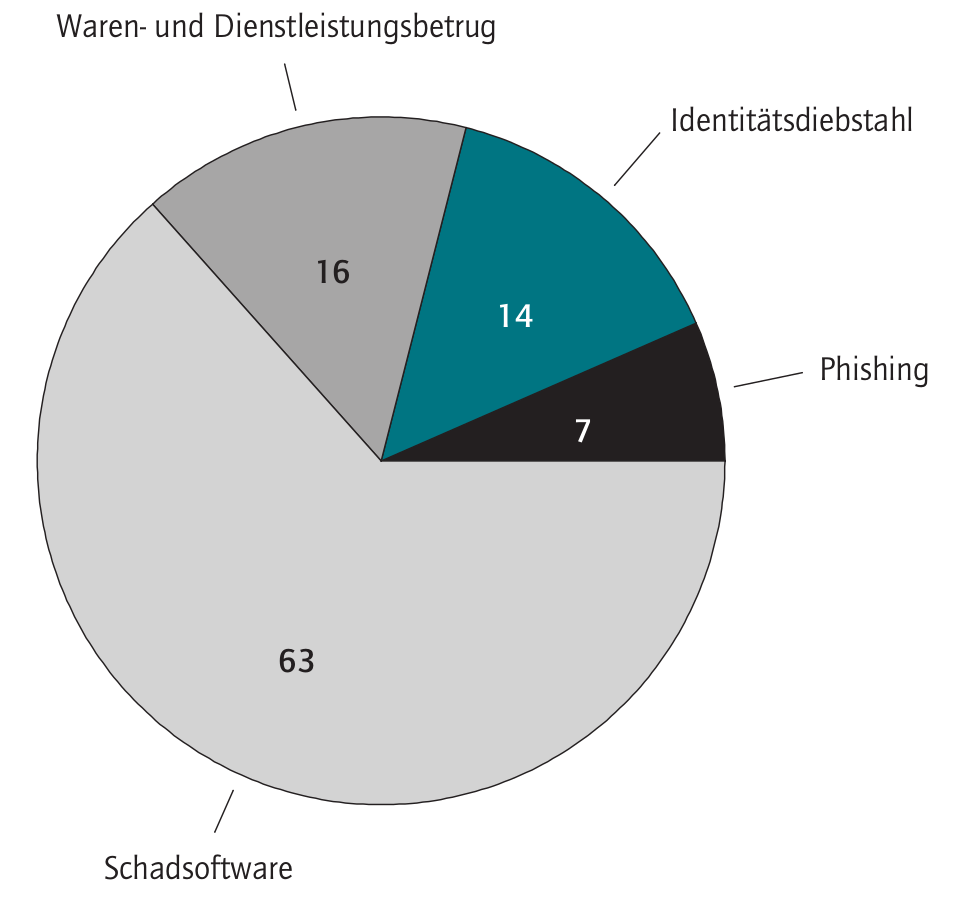
\includegraphics[width=10cm]{images/kategorien-cybercrime}
  \caption[Bedeutung der einzelnen Kategorien von Internetkriminalität]{Bedeutung der einzelnen Kategorien von Internetkriminalität\protect\footnotemark}
  \label{fig:categories-cybercrime}
\end{figure}
\footnotetext{Siehe \cite{cybercrime}, S. 297 Abbildung 1}

Abbildung \ref{fig:categories-cybercrime} zeigt die Bedeutung dieser Kategorien. Unter allen Fällen
von Internetkriminalität sind demnach 63 \% Delikte mit Schadsoftware, 16\% Betrüge im Waren-
und Dienstleistungsbereich, 14\% machen Identitätsdiebstäle aus und 7\% kommen von Phishingseiten.

In den folgenden Abschnitten werden nun einige übliche Angriffstypen von Webseiten auf den Nutzer
vorgestellt und eine mögliche Überprüfung in \textit{webifier} dargestellt.

\subsection{Malware}

Spyware, Root Kits, Trojaner und viele mehr - alles das ist Malware, welche den Nutzern in unterschiedlichen Weisen kleineren, oder größeren Schaden zuführen. Kurz: Malware ist Software mit bösartiger Wirkung. In diesem Abschnitt werden nun einige Formen von Schadsoftware beschrieben und wie diese in ein System gelangen kann.\footcite[Vgl.][95]{netzwerkDatensicherheit}

Malware ist so vielfältig wie gutartige Anwendungen. Dennoch lässt sie sich auf verschiedene Weisen
klassifizieren. Allerdings sind die Übergänge der einzelnen Klassen fließend. Zum Einen kann
Malware im Hinblick auf ihre Verbreitungsmethode und zum Anderen in der Art des Schadens für den
ungewollten Anwender unterschieden werden. Alle Klassen vereint jedoch, dass Malware im allgemeinen
Code enthält, welcher dem Nutzer oder dessen System Schaden zufügt.\footcite[Vgl.][95\psq]{netzwerkDatensicherheit}

Bei der Verbreitungsmethode kann zwischen Viren, Trojanern und Würmern unterschieden werden. Viren
sind Programme, welche sich bei der Ausführung selbst kopieren, beispielsweise indem sie ihren Code
in andere Programme oder Dokumente des Nutzers
einschleusen.\footcite[Vgl.][95]{netzwerkDatensicherheit} Die ersten Viren wurden Anfang der 1980er
Jahre in Umlauf gebracht, allerdings spielten Viren sogar schon 1970 in dem Science Fiction Film
\textit{The Scarred Man} eine Rolle.\footcite[Vgl.][14]{virusesMalware} Trojaner sind Anwendungen,
welche vortäuschen gutartig zu sein, aber Code beinhalten, welcher dem System oder dem User
schadet. Trojaner sind seit 1972 bekannt und verbreiten sich üblicherweise nicht
eigenständig.\footcite[Vgl.][12\psq]{virusesMalware} Würmer verbreiten sich üblicherweise von
alleine über Netzwerke und infizieren so andere Systeme. Hierfür nutzen sie Schwachstellen in
Netzwerkdiensten und schaden so der Maschine oder dem
Anwender.\footcite[Vgl.][95]{netzwerkDatensicherheit} Die ersten Würmer sind wie die ersten Viren
in der Science Fiction zu finden. Würmer kommen erstmals im Roman \textit{The Shockwave Rider}
von John Brunner aus dem Jahr 1975 vor. Die ersten realen Würmer waren bereits 1970 im damaligen Arpanet zu
finden.\footcite[Vgl.][15]{virusesMalware}

Anhand des angerichteten Schadens kann Malware in Spyware, Adware, Malware-Dialer, Zombie-Malware,
Backdoors und Root Kits unterteilt werden. Spyware ist Software, welche ohne Wissen des Nutzers
Informationen sammelt und weiterleitet. Dadurch können vertrauliche Daten gestohlen und missbraucht
werden.\footcite[Vgl.][95\psq]{netzwerkDatensicherheit} Solche Daten können beispielsweise
Benutzernamen und Passwörter, E-Mailadressen, Bankaccounts und Kreditkartennummern oder
Softwarelizenzschlüssel sein. Mitte der 1990er Jahre war erste Spyware zu
finden.\footcite[Vgl.][16]{virusesMalware} Als Adware werden Programme bezeichnet, welche dem
Benutzer Werbeanzeigen einblenden.\footcite[Vgl.][96]{netzwerkDatensicherheit} Adware ist ähnlich
zu Spyware, da beide Informationen über den Nutzer sammeln. Allerdings ist Adware mehr auf
Marketing fokussiert und nutzt die Informationen um dem Nutzer Webung zu
präsentieren.\footcite[Vgl.][17]{virusesMalware} Dialer sind Programme, welche Computern über
Modems oder Telefonnetze Zugang zum Internet anbieten. Malware-Dialer nutzen das aus und wählen die
Rechner ohne Kenntnis des Nutzers in teure Service-Rufnummern oder Anwahlpunkte im Ausland ein.
Allerdings wird diese Art von Malware nur noch selten genutzt, da inzwischen
telefonbasierte Internetzugänge an Bedeutung verlieren. Software, welche Rechner komprommitiert, wird als
Zombie-Malware bezeichnet, da dieser so von Angreifern ferngesteuert werden
kann.\footcite[Vgl.][96]{netzwerkDatensicherheit} Am häufigsten werden Zombie-Rechner eingesetzt um
Spam zu versenden oder mit vielen Anderen Denial of Service Angriffe
auszuführen.\footcite[Vgl.][18]{virusesMalware} Backdoors sind modifizierte Programme des Systems,
über welche Hacker Sicherheitsmechanismen umgehen und sich so unbefugten Zugriff auf den Rechner
verschaffen können. Modifizierte Softwaregruppen, welche zum Ziel haben deren Aktivität oder die
eines Angreifers vor Systembenutzern, inklusive Administratoren zu verstecken werden als Root Kits
bezeichnet.\footcite[Vgl.][96]{netzwerkDatensicherheit}

Wie Abbildung \ref{fig:malware} zeigt, nimmt die Verbreitung von Malware in Deutschland weiterhin zu
und verliert deshalb nicht an Bedeutung.

\begin{figure}[H]
  \centering
  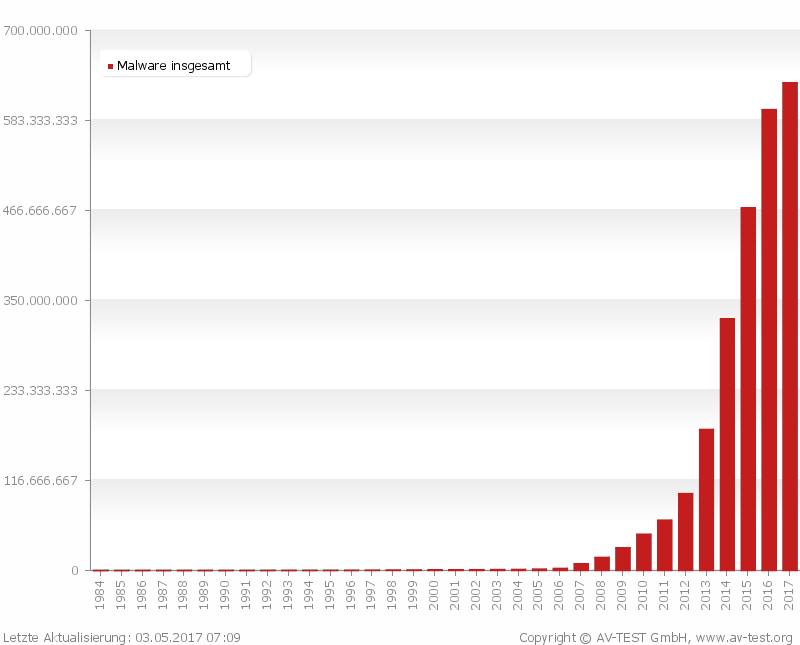
\includegraphics[width=14cm]{images/malware-all-years_sum_de}
  \caption[Malware Verbreitung in Deutschland]{Malware Verbreitung in Deutschland\protect\footnotemark}
  \label{fig:malware}
\end{figure}
\footnotetext{Siehe \cite{avtest}, Abbildung 1}

Interessant ist allerdings, dass in Abbildung \ref{fig:malware-new} ein deutlicher Rückgang in der
Verbreitung neuer Malware zu erkennen ist. Daraus lässt sich schließen, dass die bereits
in Umlauf gebrachte Schadware nach wie vor ausreicht um dem Großteil der Nutzer zu schaden.

\begin{figure}[H]
  \centering
  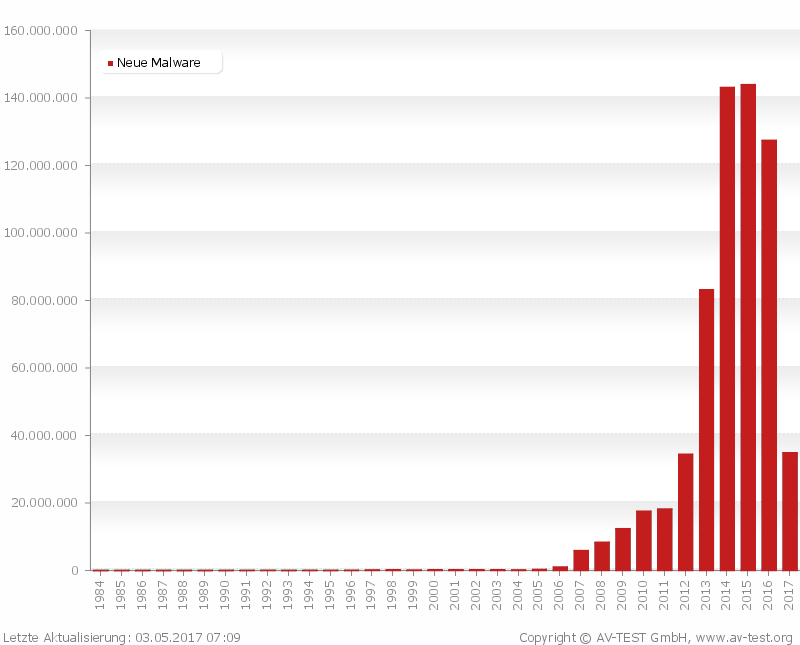
\includegraphics[width=14cm]{images/malware-all-years_de}
  \caption[Verbreitung neuer Malware in Deutschland]{Verbreitung neuer Malware in Deutschland\protect\footnotemark}
  \label{fig:malware-new}
\end{figure}
\footnotetext{Siehe \cite{avtest}, Abbildung 2}

Die Verbreitung von Malware beginnt größtenteils über Webseiten und
E-Mails.\footcite[Vgl.][97]{netzwerkDatensicherheit} Deshalb ist es notwendig mit \textit{webifier}
Webseiten auf Malware zu prüfen.


\subsection{User Agent Sniffing}
\label{sec:user-agent-sniffing}

Wer sich im \ac{WWW} bewegt benutzt meist Software, die die Navigationsbefehle des Users in
HTTP-Requests umwandeln und an den jeweiligen Webserver schicken.
Diese Programme werden \textit{User Agents} genannt.
Menschen verwenden Browseranwendungen als \textit{User Agents}, um sich auf einer grafischen
Oberfläche durch das Netz zu klicken.
Ein weitaus kleinerer, aber umso wichtigerer Teil der Websurfer sind Maschinen, die selbstständig
arbeiten: Webcrawler.
Dies sind Programme, die nach komplexen Algorithmen arbeiten, indem sie Webseiteninhalte über HTTP
herunterladen, analysieren und daraus wieder neue HTTP-Requests generieren.
\footcite[Vgl.][19]{httpGuide}
HTTP-Requests beinhalten einen Request-Header, der dem Server Auskunft über den Browser des Clients
und den gewünschten Ressourcentyp geben kann.
\footcite[Vgl.][9]{httpReference}
Das wichtigste Header-Feld zur Identifizierung heißt \textit{User Agent}. Es enthält im Normalfall
den Browsertyp, die Browserversion und das Betriebssystem, in welchem der Browser läuft, und
wird von einigen Webservern und Webanwendungen benutzt, um je nach Wert des Feldes unterschiedliche Ressourcen
zurückzuliefern.\footcite[Vgl.][259, 528\psq]{httpGuide}

Diese Technik wird \textit{User Agent Sniffing} genannt und ist ein unerwünschter Eingriff,
der nur selten seine Berechtigung hat.
Er zählt zu den Bad Pracitces in der Webentwicklung.\footcite[Vgl.][]{mdnBrowserDetection}
Das Zurückliefern unterschiedlicher Ressourcen je nach \textit{User Agent} wird in der
Fachliteratur hingegen unterschiedlich bewertet.
Gorley zeigt zunächst ein entscheidendes Problem dieses
Verhaltens auf.\footcite[Vgl.][228]{httpGuide}
Viele Webseiten passen ihre Inhalte für verschiedene \textit{User Agents} an.
Ihr Ziel ist es sicherzustellen, dass ihre Anwendungen auf möglichst allen Geräten laufen.
Funktioniert etwas nicht, weil beispielsweise die Browserversion zu alt ist, dann wird eine
Fehlerseite zurückgeliefert.
Vollautomatisierte Webcrawler bekommen häufig diese Fehlerseiten zurückgeliefert und arbeiten mit
diesen weiter, obwohl sie die Funktionen der Seiten an sich gar nicht anwenden, sondern lediglich
deren Quelltext analysieren wollen.
Im Gegensatz dazu macht er später die Aussage, dass Webserver durchaus ihre Antworten
an den \textit{User Agent} anpassen können und dies nicht so schlimm
sei.\footcite[Vgl.][402]{httpGuide}

Habe der Client einen veralteten Browser, der kein JavaScript unterstützt, so könne der
Webserver in diesem Fall einfach eine Webseite ohne JavaScript zurückliefern.
Shepherd erläutert drei Hauptgründe, warum \textit{User Agent Sniffing}
betrieben wird: Bug-Workarounds, Feature-Unterstützung und Browserspezifisches
HTML.\footcite[Vgl.][]{mdnBrowserDetection} Da es für all diese Beweggründe bessere Lösungsansätze
gibt und \textit{User Agent Sniffing} als Vorstufe zum Browserexploit genutzt werden kann, wird es
in dieser Arbeit als Angriff auf den Client angesehen.


\subsection{JavaScript Port \& IP Scanning}
Um Angriffe über das Netzwerk zu starten muss der Angreifer Kenntnisse über den Netzwerkaufbau und
die erreichbaren Services des anzugreifenden Systems haben.\footcite[Vgl.][937]{port1}

Über die offenen Ports eines Systems kann sich ein potenzieller Angreifer Zugang beschaffen. Jedoch
muss zunächst herausgefunden werden, welche Ports erreichbar sind. Hierfür wird eine Technik Namens
\textit{Port Scanning} genutzt. Port Scanning ist im Grunde das Abfragen einiger oder auch aller
Ports eines Systems. Es gibt derzeit 65.535 TCP und 65.535 UDP Ports, von denen einige in
Systemen offen, jedoch die meisten davon geschlossen sind.\footcite[Vgl.][937]{port1} UDP und TCP
sind zwei verschiedene Internet Protokolle. Sie unterscheiden sich zum Einen darin, dass TCP
verbindungsorientiert arbeitet, während UDP verbindungslose Kommunikation
nutzt.\footcite[Vgl.][]{tcpudp} Ein Portscanner nutzt die verschiedenen Eigenschaften der
Protokolle aus um festzustellen ob ein Port offen oder geschlossen ist.\footcite[Vgl.][31]{port2}
Die Unterschiede werden hier aber nicht weiter beleuchtet. Einige dieser Ports sind standardisiert
und werden von bestimmten Webservices genutzt, wie beispielsweise TCP Port 80, welcher in der Regel
von Web Servern eingesetzt wird.

Port Scanning liefert hierbei Informationen welche Ports eines Systems offen für Netzwerkverbindungen sind.

In Listing \ref{lst:portscanner} wird ein Beispielcode für einen, in Java implementierten, simplen Portscanner gezeigt. Dieser prüft alle 65535 TCP Ports eines gegebenen Hosts. Er versucht über jeden dieser Ports eine Socketverbindung aufzubauen (siehe Zeile 19-32), welche er anschließend wieder schließt. Wenn hierbei keine Fehlermeldung vom System geworfen wird weiß der Scanner, dass die Verbindung mit dem getesteten Port aufgebaut wurde und somit dieser Port offen ist. Dieser Portscanner liefert als Ergebnis eine Anzahl an offenen Ports im getesten System.

\newpage
\begin{scriptsize}
\lstset{
    style=eclipsejava,
    caption=[Beispiel eines simplen Java PortScanners]{Beispiel eines simplen Java PortScanners\protect\footnotemark},
    label={lst:portscanner}
}
\begin{lstlisting}
public class Portscanner {
    public static void main(final String... args) {
        final ExecutorService es = Executors.newFixedThreadPool(20);
        final String ip = "127.0.0.1";
        final int timeout = 200;
        final List<Future<Boolean>> futures = new ArrayList<>();
        for (int port = 1; port <= 65535; port++) {
            futures.add(portIsOpen(es, ip, port, timeout));
        }
        es.shutdown();
        int openPorts = 0;
        for (final Future<Boolean> f : futures) {
            if (f.get()) {
                openPorts++;
            }
        }
        System.out.println("There are " + openPorts + " open ports on host " + ip + " (probed with a timeout of " + timeout + "ms)");
    }
    
    public static Future<Boolean> portIsOpen(final ExecutorService es, final String ip, final int port, final int timeout) {
        return es.submit(new Callable<Boolean>() {
            @Override public Boolean call() {
                try {
                    Socket socket = new Socket();
                    socket.connect(new InetSocketAddress(ip, port), timeout);
                    socket.close();
                    return true;
                } catch (Exception ex) {
                    return false;
                }
            }
        });
    }
}
\end{lstlisting}
\end{scriptsize}
\footnotetext{Zitat \cite{portscanner}}

Es gibt grundsätzlich viele verschiedene Möglichkeiten ein Angriffsziel auf offene Ports zu
überprüfen. Die in Codebeispiel \ref{lst:portscanner} gezeigte Möglichkeit ist relativ simpel,
aber effektiv.
Jedoch ist es ebenfalls einfach einen derartigen Angriff zu blockieren, da Schutzprogrammen leicht
erkennen können, dass es sich um einen Portscan-Angriff handelt und die entsprechende IP dann für
weitere Anfragen sperren. Um diesen offensichtlichen Angriff zu verschleiern werden oft verschiedene
Hosts genutzt. Der Angriff verteilt sich auf Anfragen von verschiedenen IP's, was es einem
Erkennungsalgorithmus erschwert legitime Anfragen von einem verteilten Portscan zu differenzieren.
Je mehr Hosts an einem derartigen Scan beteiligt sind, desto schwieriger wird es den entsprechenden
Scan zu erkennen und entsprechende IP's zu blockieren. Zusätzlich spielt noch die Art der Anfrage
eine Rolle. Es kann beispielsweise mittels eines Pings ein bestimmter Port angefragt werden. Dies
ist aber keine effiziente Methode, da Firewalls Pings oft blockieren.

Im Folgenden wird einer der bekanntesten Scantypen, der SYN-Scan, erläutert. Für das Verständnis
eines SYN-Scans muss zunächst erklärt werden, wie in TCP Verbindungen aufgebaut werden.

TCP nutzt für den Verbindungsaufbau den 3-Wege-Handshake. Der Ablauf ist in Abbildung
\ref{fig:handshake} dargestellt. Zuerst sendet der Client einen \textit{SYN} an den Server. Dieser
wird dann vom Server empfangen und er sendet einen \textit{ACK} als Antwort und gleichzeitig einen
eigenen \textit{SYN} zurück an den Client. Zum Schluss sendet der Client noch einen \textit{ACK}
zum Server als Antwort auf dessen \textit{SYN}. Die Verbindung ist danach aufgebaut und es können
Daten übermittelt werden.\footcite[Vgl.][32]{port2} \begin{figure}[H]
  \centering
  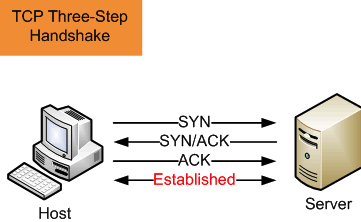
\includegraphics[width=10cm]{images/handshake}
  \caption[3-Step-Handshake TCP]{3-Step-Handshake TCP\protect\footnotemark}
  \label{fig:handshake}
\end{figure}
\footnotetext{Siehe \cite{handshake}, Abbildung 1}

Bei einem SYN-Scan versucht nun der Angreifer TCP-Verbindungen über die zu scannenden Ports
aufzubauen. Er sendet also SYN-Anfragen an diese. Anhand der Antwort kann der Scanner den Status
des Ports erkennen. Antwortet das Angriffsziel mit einem SYN/ACK so ist der Port offen. Ist die
Antwort ein Reset-Flag(RST), kann der Port als geschlossen markiert werden. Komplizierter wird es,
wenn keine Antwort kommt. Dies kann mehrere Gründe haben. Zum Einen ist es möglich, dass das
Angriffsziel keine Verbindung hat. Deshalb sollte vor dem Scan überprüft werden ob der Rechner
erreichbar ist. Ein weiterer Grund könnte eine Firewall sein, die Anfragen blockiert. Um dies
herauszufinden wird das SYN-Packet wiederholt gesendet, falls keine Antwort zurückkommt. Ist ein
Server erreichbar, aber es folgt keine Antwort auf einen SYN kann der Port als gefiltert markiert
werden, was aussagt, dass eine Firewall die Verbindungen blockiert.\footcite[Vgl.][33]{port2}

Um als Webseite die eigenen Nutzer zu scannen muss der Portscan-Code beispielsweise mittels
JavaScript in die Seite eingebunden werden. Hier gibt es verschiedene Arten den Code möglichst
unauffällig zu platzieren. Eine Möglichkeit wird in Listing \ref{lst:javascriptscanner} gezeigt.
Hier wird Portscanning betrieben indem versucht wird von der entsprechenden IP und dem Port eine
img-Datei nachzuladen. Je nach Ergebnis wird dann entschieden ob der Port offen oder geschlossen
ist. Bei erfolgreichem Laden oder einer Fehlermeldung bedeutet es, dass der Port offen ist, da er
reagiert. Läuft der Request in einen Timeout wird der Port als geschlossen angesehen.

Für die Funktion müssen die Host-Adresse, der zu scannende Port und ein Timeout-Wert übergeben
werden.
Zunächst wird nun ein neues Image-Objekt erstellt (Zeile 2). Es wird definiert, dass bei einem
Fehler als Rückgabewert oder einem erfolgreichen Laden der Port als offen markiert wird (Zeile 4-9).
Bei bestimmten Ports muss noch das Protokoll entsprechend geändert werden. Beispielsweise muss für
Port 443 das HTTPS-Protokoll verwendet werden (Zeile 16). Als Standardprotokoll ist HTTP
definiert (Zeile 17). Das Protokoll, die Host-Adresse und der Port bilden zusammen den Pfad für das
Image-Objekt. Je nach Protokoll muss noch ein eine Bildressource angegeben werden (Zeile 17). Als
Name der Bilddatei wird hier die ID verwendet. Dieser Name ist jedoch irrelevant. Zum Schluss wird
bei einem Timeout der Port als geschlossen markiert (Zeile 20-24). Mithilfe der Function
\lstinline[style=eclipse]{scan()} wird der Portscan gestartet. Listing \ref{lst:javascriptscanner}
bildet nur einen Teil des Portscans ab, zur besseren Übersichtlichkeit wurden Initialisierung von Host und
Port-Bereich sowie die Ergebnisausgabe nicht dargestellt.

\newpage
\begin{scriptsize}
\lstset{
    style=eclipsejavascript,
    caption=[Beispiel eines simplen JavaScript PortScanners]{Beispiel eines simplen JavaScript PortScanners},
    label={lst:javascriptscanner}
}
\begin{lstlisting}
function scan(){
   var  req = new pingrequest( f.host.value,p,t);
   req.dorequest();
}
this.dorequest = function() {
   var img = new Image();

   img.onerror = function () {
      if (!img) return;
      img = undefined;
      callback( host, port, 'up',id);
   };
   img.onload = img.onerror;

   switch(port){
      case 21:  src = 'ftp://' + this.id() + '@' + host + '/'; break;//ftp
      case 25:  src = 'mailto://' + this.getid() + '@' + host ; break;//smtp **
      case 70:  src = 'gopher://' + host + '/'; break;//gopher
      case 119: src = 'news://' + host + '/'; break;//nntp **
      case 443: src = 'https://' + host + '/' + this.getid() + '.jpg';
      default:  src = 'http://' + host + ':' + port + '/' + this.getid() + '.jpg';// getid is here to prevent cache seekings;
   }
   img.src = src;
   setTimeout(function () {
      if (!img) return;
      img = undefined;
      callback( host, port, 'down',id);
   }, timeout);
};
\end{lstlisting}
\end{scriptsize}

Zusätzlich zum Portscan gibt es noch den IP-Scan. Ein IP-Scan funktioniert grundsätzlich ähnlich
zum Portscan. Hier wird jedoch nicht versucht die möglichen Angriffspunkte eines Rechners
aufzudecken, sondern das Netzwerk auszuspähen. Da JavaScript clientseitig ausgeführt wird, versuchen
Angreifer häufig über die bekannten \textit{Heimnetz-IPs} (beispielsweise. 192.168.178.*) das
Netzwerk zu analysieren. Es werden die IP-Bereiche nach anderen Rechner abgesucht, die sich in dem
Netzwerk befinden. So kann ein Angreifer Erkenntnisse über das komplette Netzwerk seines Ziels
erlangen um so einen erfolgreicheren Angriff zu starten.

\subsection{Phishing}

Beim Phishing versucht ein Angreifer, in diesem Fall auch Phisher genannt, auf betrügerische Weise
vertrauliche oder sensible Anmeldedaten zu bekommen. Um dies zu erreichen fälscht er die
elektronische Kommunikation zwischen Opfer und einer vertrauenswürdigen oder öffentlichen
Organisation, indem er sich selbst als diese ausgibt. Dies geschieht meist durch E-Mails, welche
das Opfer auf eine Webseite locken, die vermeindlich zur vertrauenswürdigen Organisation gehört,
in Wahrheit aber vom Angreifer kontrolliert wird und deshalb Informationen, vorzugsweise Passwörter
oder Kreditkartennummern abfängt.\footcite[Vgl.][1]{phishing}

Phishing gibt es seit Anfang der 1990er Jahre, allerdings sind die Zahlen von Phishing-Angriffen in
den letzten Jahren drastisch gestiegen. Phishing ist zu einer gefährlichen Kombination aus Social
Engeneering und technischen Angriffen geworden, welche zum Ziel hat vertrauliche Informationen zu
erlangen. Die gewonnenen Daten werden für Betrug, Identitätsdiebstahl und Spionage missbraucht.
\footcite[Vgl.][1\psq]{phishing}

Im Folgenden wird ein beispielhafter Phishingangriff auf PayPal geschildert. PayPal ist ein
Online-Bezahldienst mit über 18 Millionen Nutzern alleine in Deutschland. \footcite[Vgl.][]{paypal}
Am häufigsten wird PayPal genutzt um Internetkäufe zu bezahlen. Listing \ref{lst:phishing-mail}
zeigt eine E-Mail, mit der ein PayPal-Nutzer auf eine Phishing-Seite gelockt werden
soll.\footcite[Vgl.][10]{phishing}

\newpage

\begin{scriptsize}
\lstset{
    style=nonumbers,
    caption=[Phishing Lockmail]{Phishing Lockmail\protect\footnotemark},
    label={lst:phishing-mail}
}
\begin{lstlisting}
Sehr geehrter PayPal-Kunde, sehr geehrte PayPal-Kundin,

wir haben gerade einen oder mehrere Loginversuche von einer fremden IP-Adresse auf Ihr
PayPal-Konto festgestellt.

Wenn Sie in der letzten Zeit unterwegs auf Ihren Account zugegriffen haben, könnten die
ungewöhlichen Loginversuche von Ihnen stammen. Vorallem wenn die Loginversuche nicht von Ihnen
stammen, besuchen Sie PayPal bitte sobald wie möglich um Ihre Identität zu verifizieren:

(*https://www.paypal.com/signin?country.x=DE&locale.x=de_DE*)

Die Bestätigung Ihrer Identität ist eine Sicherheitsmaßnahme, mit der sichergestellt wird,
dass Sie die enzige Person sind, die Zugriff auf Ihr Konto hat.

Vielen Dank für Ihre Unterstützung um gemeinsam Ihr Konto zu schützen.

Mit freundlichen Grüßen,
PayPal
-------------------------------------------------------------------------
                        SCHÜTZEN SIE IHR PASSWORT

Geben Sie ihr Passwort niemals an Dritte weiter und nutzen Sie es ausschließlich um sich auf
(*https://www.paypal.com/*) anzumelden. Schützen Sie sich vor Betrug, indem Sie einen
neuen Browser öffnen und jedes mal die PayPal Url eintippen um sich anzumelden.
-------------------------------------------------------------------------

Bitte antworten Sie nicht auf diese E-Mail. Nachrichten, die an diese Adresse gesendet werden
können nicht beantwortet werden. Wenn Sie Hilfe benötigen melden Sie sich in Ihrem
PayPal-Konto an und klicken Sie auf den Hilfe-Link im Menü. 

PayPal E-Mail ID PP321
\end{lstlisting}
\end{scriptsize}
\footnotetext{Zitat \cite{phishing}, S. 11 Abbildung 1.4, Übersetzung Samuel Philipp}

Die in Listing \ref{lst:phishing-mail} dargestellte E-Mail täuscht dem Kontoinhaber vor, dass eine
Fremde Person auf das Konto zugegriffen hat und animiert ihn so dazu dem vermeindlich sicheren Link
zu folgen um seine Identität zu verifizieren und seinen Account zu schützen. Nebenbei sei noch
erwähnt, dass der Link in der E-Mail natürlich nicht auf die orginale PayPal-Webseite verweist,
sondern auf die Phishing-Seite des Angreifers. Der Hinweis \enquote{Schützen Sie Ihr Passwort}
verleiht der E-Mail noch ein authentischeres Aussehen und würde der Nutzer dem Rat folgen wäre
dieser Phishing-Angriff wirkungslos. Viele Nutzer nehmen diesen Rat auch wahr, nutzen aber trotzdem
den bereitgestellten Link aus der E-Mail, da diese ja offensichtlich von PayPal stammt und deshalb
vertrauenswürdig ist.\footcite[Vgl.][10]{phishing}

Üblicherweise wird auch die Absenderadresse der E-Mail gefälscht und eine Orginaladresse von
PayPal, beispielsweise \textit{service@paypal.com} verwendet. Wenn der Empfänger der E-Mail nun den
Link aus selbiger öffnet wird er auf die in Abbildung \ref{fig:paypal-phishing-site} dargestellte
Webseite geleitet, welche Ihn zur Eingabe seiner Anmeldedaten auffordert.\footcite[Vgl.][10]{phishing}

\begin{figure}[H]
  \centering
  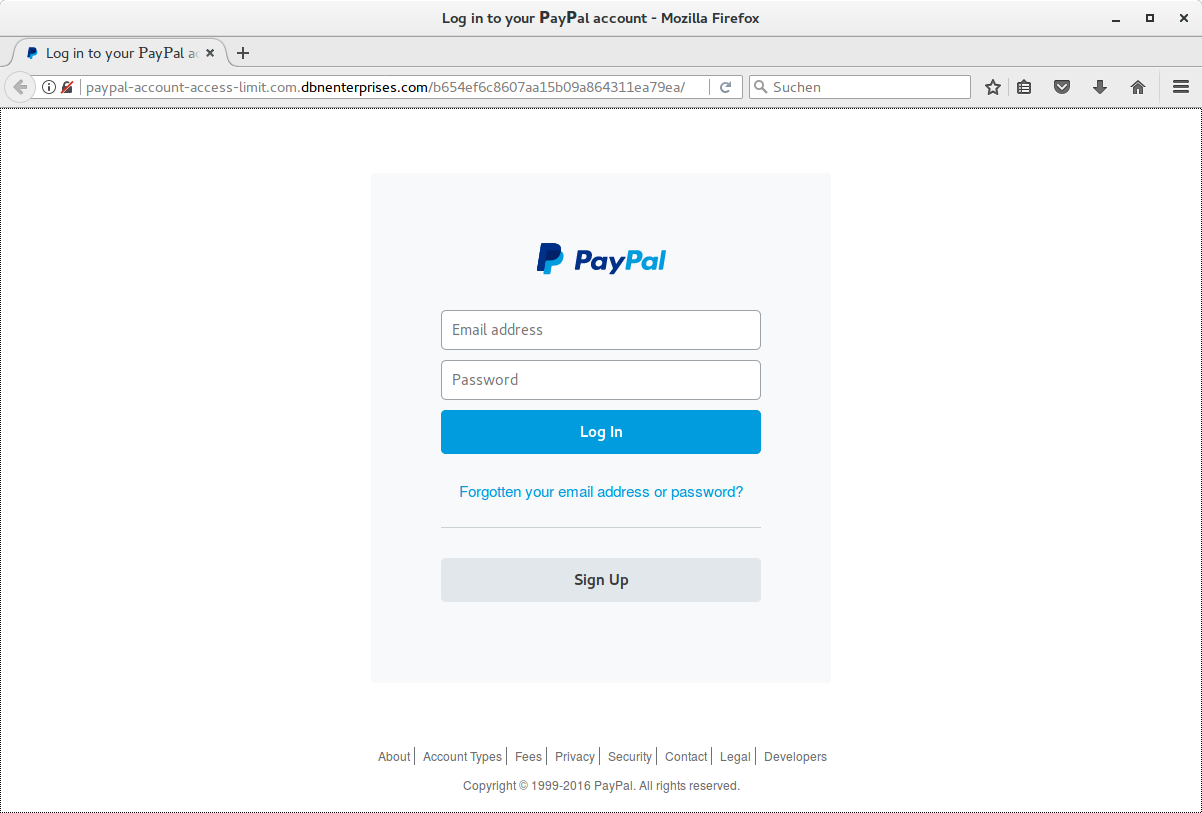
\includegraphics[width=15cm]{images/paypal-phishing-site}
  \caption{PayPal Phishing Webseite}
  \label{fig:paypal-phishing-site}
\end{figure}

Das Aussehen der Phishing-Webseite ist dem des Originals (Abbildung \ref{fig:paypal-original-site})
sehr ähnlich. Wenn das Opfer nun seinen Benutzernamen und sein Passwort eingegeben hat ist das erste
Ziel des Angreifers bereits erreicht, denn er hat gültige Zugangsdaten zu einem PayPal-Account
erhalten. Um aber noch mehr Daten zu bekommen und dem Opfer den Angriff weiterhin zu verschleiern
wird der Nutzer in vielen Fällen auf einer nachfolgenden Seite gebeten auch noch seine Anschrift
und Kreditkartendaten zu bestätigen, indem er diese eingeben muss. Danach wird der Nutzer
wieder \enquote{abgemeldet} und anschließend auf die orginale PayPal-Webseite (Abbildung
\ref{fig:paypal-original-site}) weitergeleitet. Damit ist der Phishing-Angriff abgeschlossen und
der Angreifer wird keine Zeit verlieren die Daten zu missbrauchen.\footcite[Vgl.][10\psqq]{phishing}

\begin{figure}[H]
  \centering
  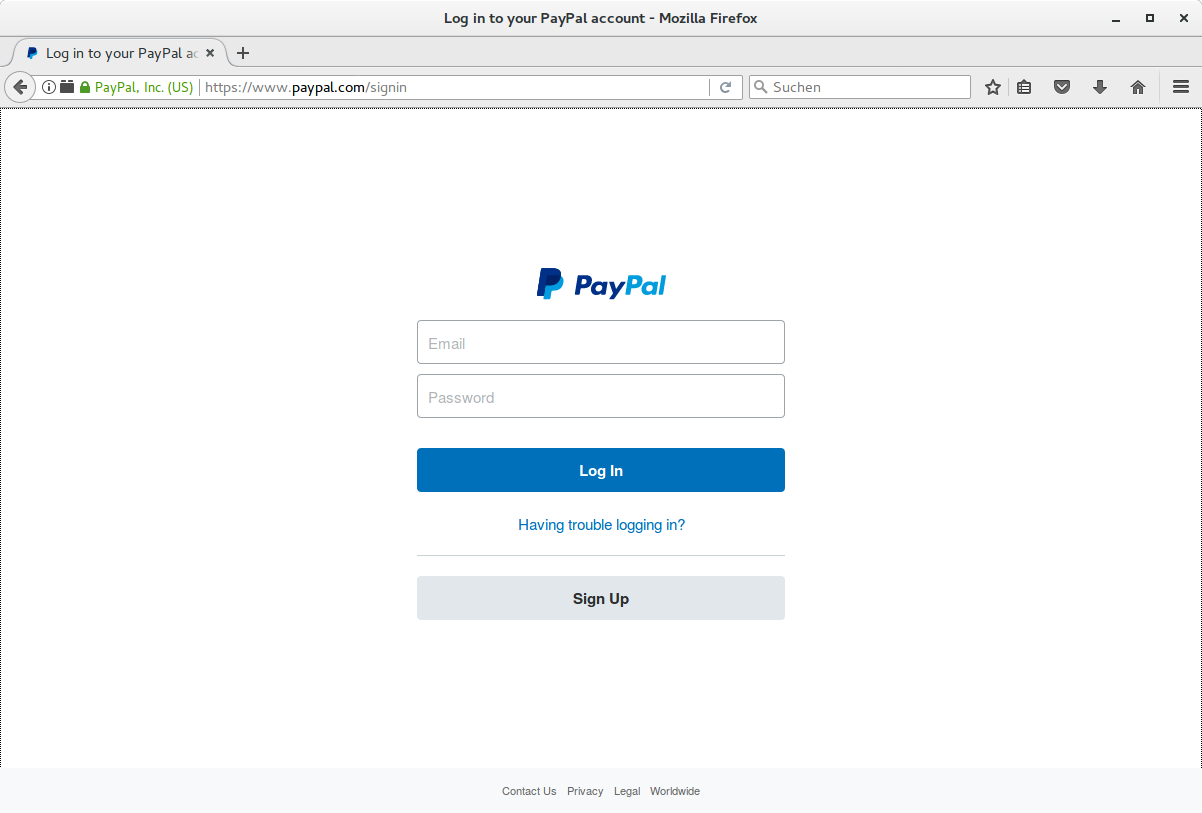
\includegraphics[width=15cm]{images/paypal-original-site}
  \caption{PayPal Original Webseite}
  \label{fig:paypal-original-site}
\end{figure}

Das Vorgehen im vorausgegangen Beispiel ist sehr typisch für Phishing-Angriffe und kann deshalb auf
sehr viele andere Seiten übertragen werden.
